\section{Experiments}

\subsection{Search Performance}

\begin{frame}
    \frametitle{Experiment I: Search Performance}

    \begin{itemize}
        \item Compare to simple reference behaviors (baselines).
        \item Test on held out environment samples.
        \item Metrics:
        \begin{enumerate}
            \item Average search path length.
            \item Average success rate.
            \item Success weighted by inverse path length (SPL)~\cite{anderson_evaluation_2018}.
        \end{enumerate}
    \end{itemize}

    \begin{definition}
        \begin{equation*}
            \text{SPL} = \frac{1}{N} \sum_{i=1}^N S_i \frac{l_i}{\max(p_i,l_i)}
        \end{equation*}
        where \(N\) is number of test samples, \(S_i\) is binary success indicator, \(p_i\) is the taken path length \(l_i\) is the shortest path length.
    \end{definition}

    % How good was the taken search path compared to the optimal search path?
    % How good a path is depends on the environment --
    % if targets are close together, a good path should be short.
    % SPL is 1.0 of the agent takes the optimal path in all test samples
    % SPL is 0.5 if the agent takes the optimal path but is only successful in half of the tests.
    % etc.
\end{frame}

\begin{frame}
    \frametitle{Baselines}

    % Simple handcrafted policies.
    % Give a sense of the performance achieved by learning agents.
    % All indicate automatically when target visible.

    \begin{description}
        \item [Random:] randomly samples actions.
        \item [Greedy:] greedily selects exploring actions (random if none).
        \item [Exhaustive:] exhaustively covers search space with minimal revisits.
        \item [Human:] human searcher with knowledge of environment.
        \item[Handcrafted:] prioritize actions that lead to higher blue intensity\\ (gaussian environment only).
    \end{description}
\end{frame}

%\movie[externalviewer]{\includegraphics{../videos/gaussian/map/0.gif}}{videos/gaussian/map/0.gif}

\begin{frame}
    \begin{table}
        \centering
        Gaussian Environment\par\vspace{0.5em}
        \begin{tabular}{lccc}
    \toprule
    Agent & SPL & Success & Length \\
    \midrule
    random & $0.06 \pm 0.01$ & $0.92 \pm 0.06$ & $369.07 \pm 24.93$\\
    greedy & $0.17 \pm 0.00$ & $1.00 \pm 0.00$ & $147.12 \pm 2.38$\\
    exhaustive & $0.21 \pm 0.00$ & $1.00 \pm 0.00$ & $83.37 \pm 2.88$\\
    handcrafted & $0.33 \pm 0.00$ & $1.00 \pm 0.00$ & $65.20 \pm 1.41$\\
    human & $0.23 \pm 0.03$ & $1.00 \pm 0.00$ & $80.97 \pm 13.49$\\
    temporal & $0.24 \pm 0.03$ & $0.99 \pm 0.01$ & $101.25 \pm 13.32$\\
    spatial & $0.29 \pm 0.02$ & $0.99 \pm 0.01$ & $72.16 \pm 5.97$\\
    \bottomrule
\end{tabular}

    \end{table}


    \begin{center}
        %\href{run:videos/gaussian/map/0.gif}{video 1}, \href{run:videos/gaussian/map/0.gif}{video 2}, \href{run:videos/gaussian/map/2.gif}{video 3} (spatial)
    \end{center}
\end{frame}

\begin{frame}
    \begin{columns}
        \begin{column}{0.55\textwidth}
            \begin{figure}
                \centering
                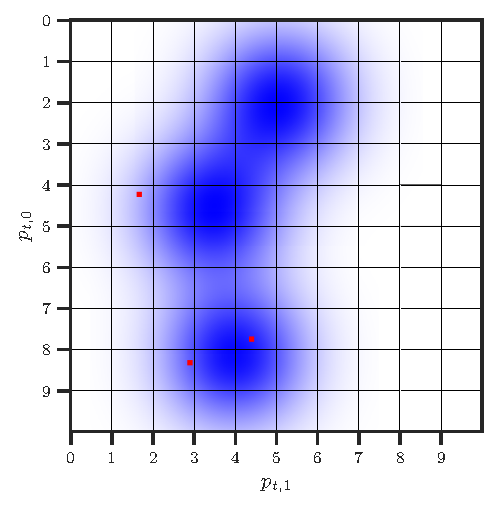
\includegraphics[scale=0.5]{figures/path-scene.pdf}
                \par Environment sample
            \end{figure}
        \end{column}
        \begin{column}{0.5\textwidth}
            \begin{figure}
                \centering
                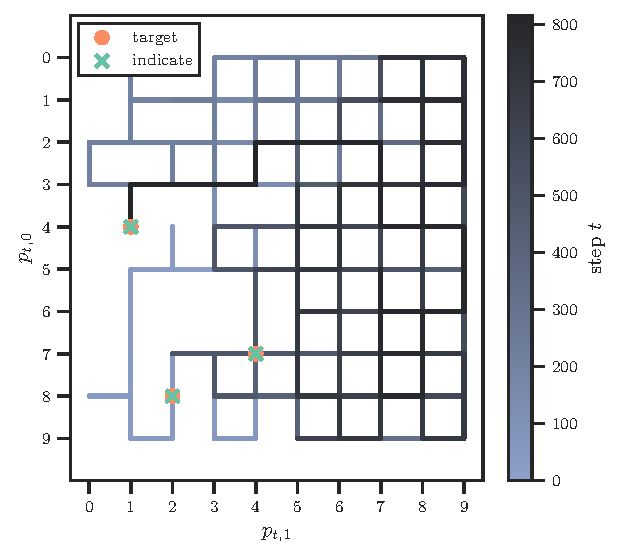
\includegraphics[scale=0.5]{figures/path-random.pdf}
                \par Random baseline
            \end{figure}
        \end{column}
    \end{columns}
\end{frame}

\begin{frame}
    \begin{columns}
        \begin{column}{0.55\textwidth}
            \begin{figure}
                \centering
                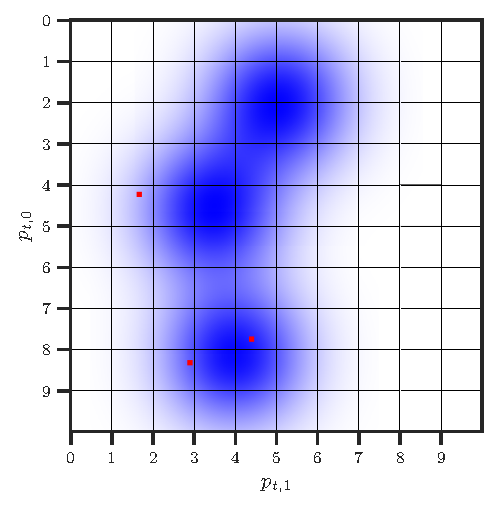
\includegraphics[scale=0.5]{figures/path-scene.pdf}
                \par Environment sample
            \end{figure}
        \end{column}
        \begin{column}{0.5\textwidth}
            \begin{figure}
                \centering
                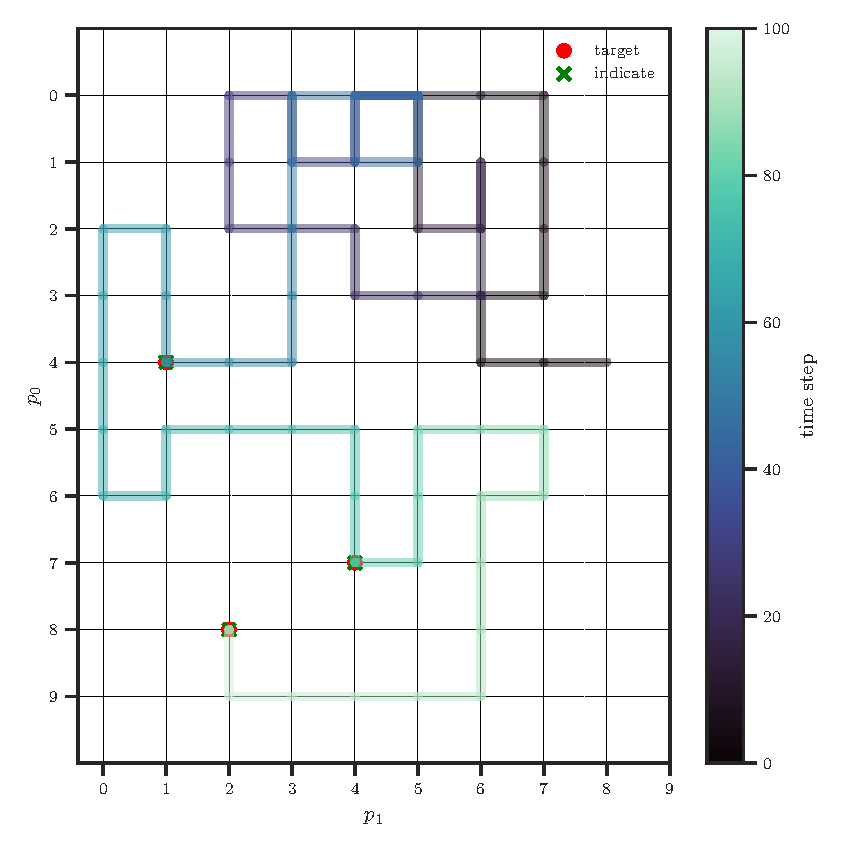
\includegraphics[scale=0.5]{figures/path-greedy.pdf}
                \par Greedy baseline
            \end{figure}
        \end{column}
    \end{columns}
\end{frame}

\begin{frame}
    \begin{columns}
        \begin{column}{0.55\textwidth}
            \begin{figure}
                \centering
                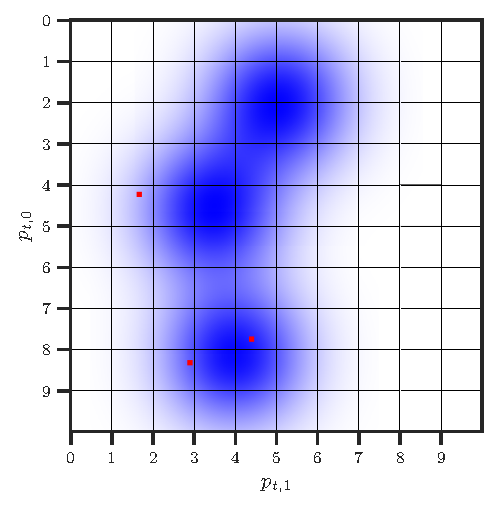
\includegraphics[scale=0.5]{figures/path-scene.pdf}
                \par Environment sample
            \end{figure}
        \end{column}
        \begin{column}{0.5\textwidth}
            \begin{figure}
                \centering
                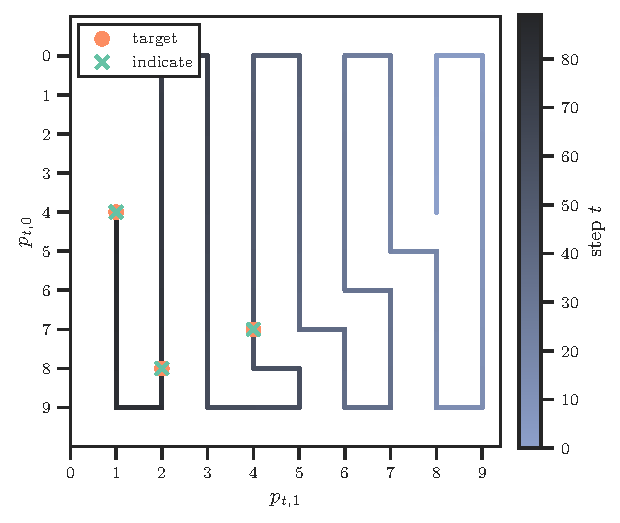
\includegraphics[scale=0.5]{figures/path-exhaustive.pdf}
                \par Exhaustive baseline
            \end{figure}
        \end{column}
    \end{columns}
\end{frame}

\begin{frame}
    \begin{columns}
        \begin{column}{0.55\textwidth}
            \begin{figure}
                \centering
                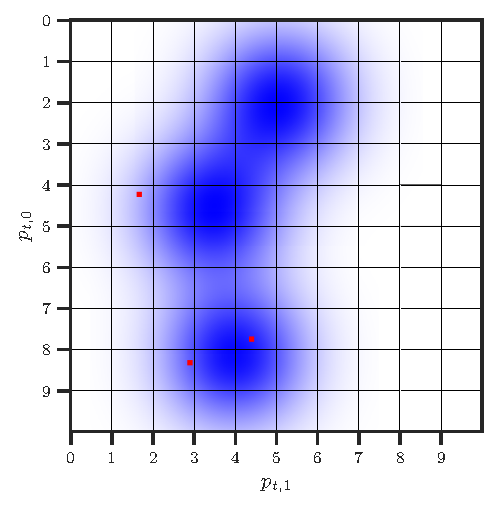
\includegraphics[scale=0.5]{figures/path-scene.pdf}
                \par Environment sample
            \end{figure}
        \end{column}
        \begin{column}{0.5\textwidth}
            \begin{figure}
                \centering
                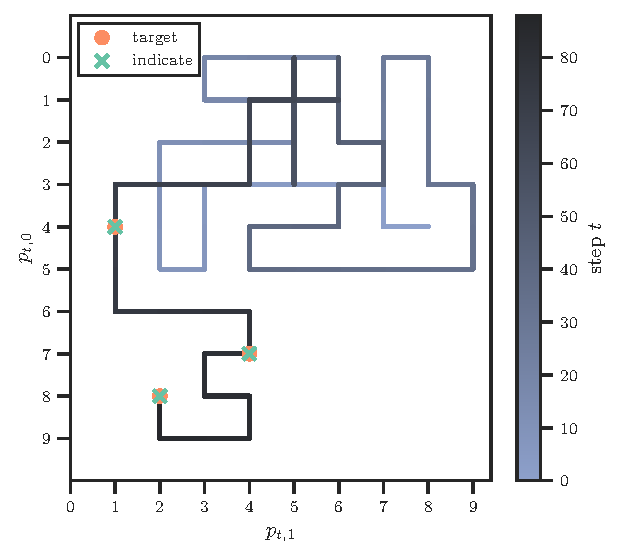
\includegraphics[scale=0.5]{figures/path-handcrafted.pdf}
                \par Handcrafted baseline
            \end{figure}
        \end{column}
    \end{columns}
\end{frame}

\begin{frame}
    \begin{columns}
        \begin{column}{0.55\textwidth}
            \begin{figure}
                \centering
                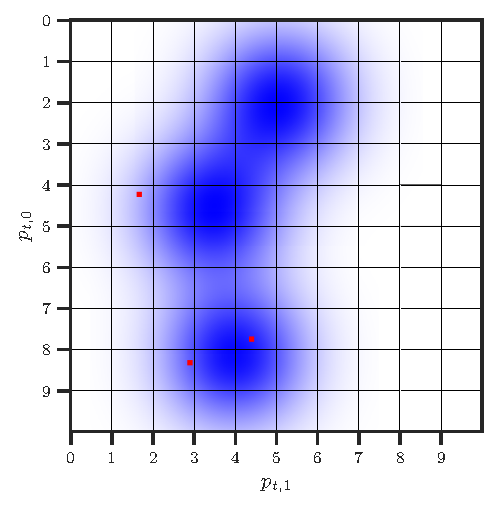
\includegraphics[scale=0.5]{figures/path-scene.pdf}
                \par Environment sample
            \end{figure}
        \end{column}
        \begin{column}{0.5\textwidth}
            \begin{figure}
                \centering
                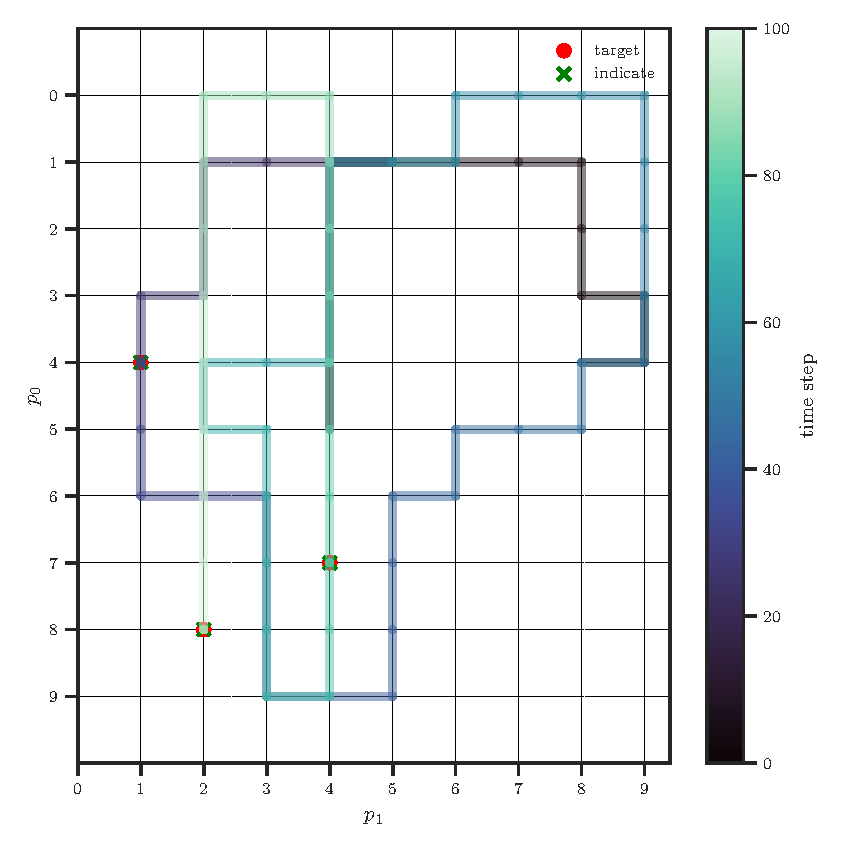
\includegraphics[scale=0.5]{figures/path-lstm.pdf}
                \par Temporal memory
            \end{figure}
        \end{column}
    \end{columns}
\end{frame}

\begin{frame}
    \begin{columns}
        \begin{column}{0.55\textwidth}
            \begin{figure}
                \centering
                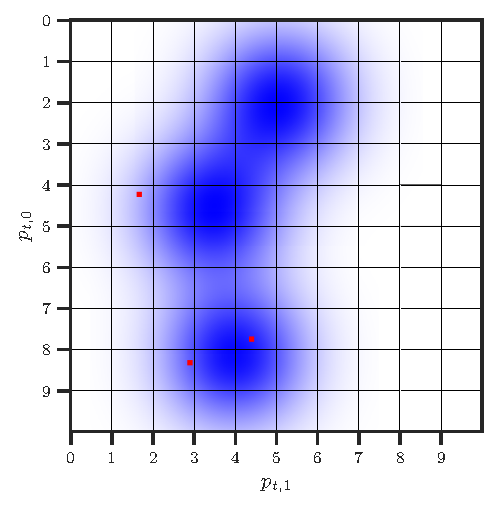
\includegraphics[scale=0.5]{figures/path-scene.pdf}
                \par Environment sample
            \end{figure}
        \end{column}
        \begin{column}{0.5\textwidth}
            \begin{figure}
                \centering
                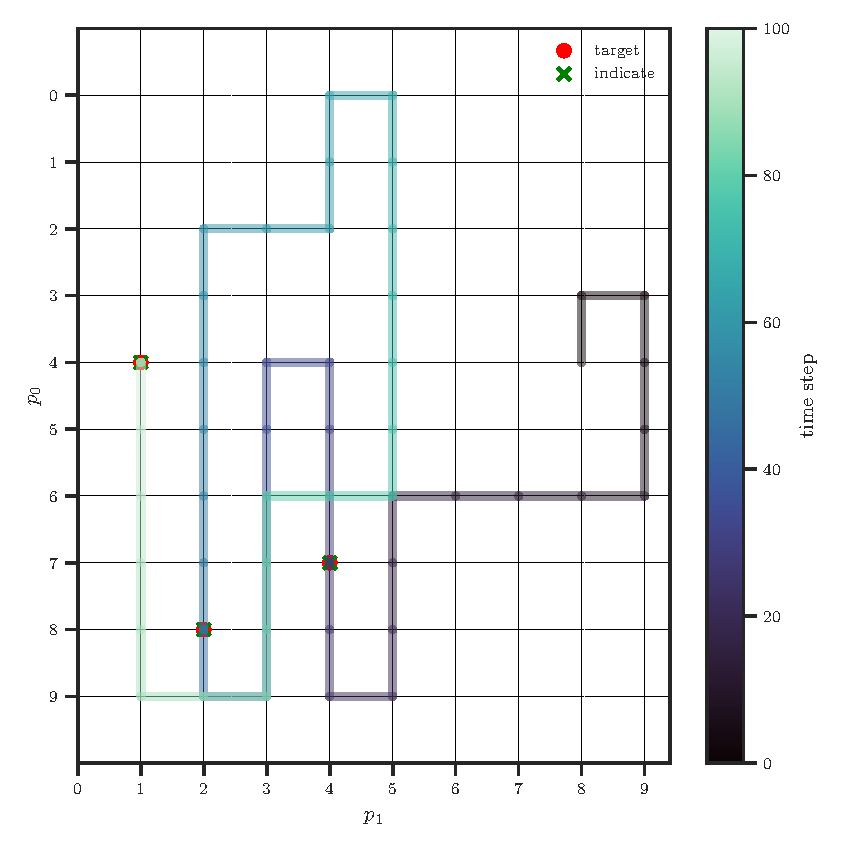
\includegraphics[scale=0.5]{figures/path-map.pdf}
                \par Spatial memory 
            \end{figure}
        \end{column}
    \end{columns}
\end{frame}

\begin{frame}
    \begin{figure}
        \centering
        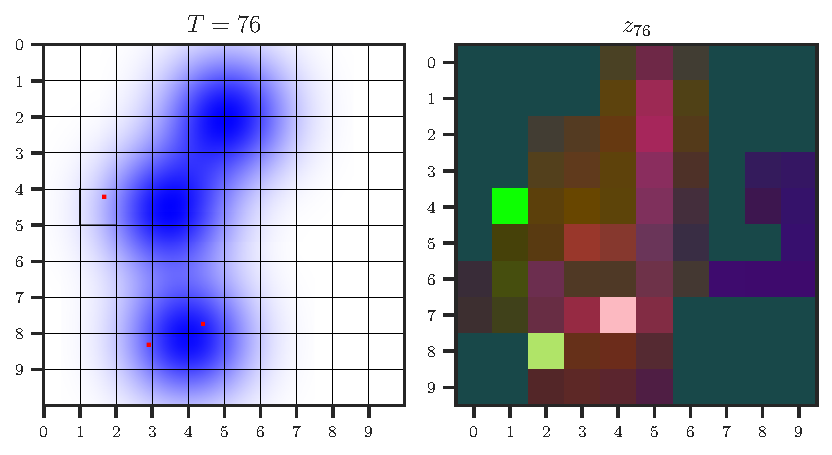
\includegraphics[scale=0.75]{figures/memory-map.pdf}
        \par PCA decomposition of spatial memory after episode.
    \end{figure}
\end{frame}

\begin{frame}
    \begin{table}
        \centering
        Terrain Environment\par\vspace{0.5em}
        \begin{tabular}{lccc}
    \toprule
    Agent & SPL & Success & Length \\
    \midrule
    random & $0.06 \pm 0.01$ & $0.89 \pm 0.04$ & $366.05 \pm 26.96$\\
    greedy & $0.17 \pm 0.01$ & $1.00 \pm 0.00$ & $141.01 \pm 2.31$\\
    exhaustive & $0.22 \pm 0.00$ & $1.00 \pm 0.00$ & $84.11 \pm 0.84$\\
    human & $0.26 \pm 0.02$ & $1.00 \pm 0.00$ & $76.73 \pm 5.33$\\
    \midrule
    temporal & $0.25 \pm 0.02$ & $1.00 \pm 0.01$ & $103.76 \pm 11.69$\\
    spatial & $0.27 \pm 0.01$ & $1.00 \pm 0.00$ & $79.60 \pm 6.88$\\
    \bottomrule
\end{tabular}
    \end{table}

    \centering \href{run:videos/terrain/map/0.gif}{video 1}, \href{run:videos/terrain/map/0.gif}{video 2}, \href{run:videos/terrain/map/2.gif}{video 3} (spatial)
\end{frame}

\begin{frame}
    \begin{table}
        \centering
        Camera Environment\par\vspace{0.5em}
        \begin{tabular}{lccc}
    \toprule
    Agent & SPL & Success & Length \\
    \midrule
    random & $0.04 \pm 0.00$ & $0.62 \pm 0.03$ & $545.09 \pm 56.25$\\
    greedy & $0.12 \pm 0.01$ & $0.97 \pm 0.01$ & $255.60 \pm 10.44$\\
    exhaustive & $0.37 \pm 0.00$ & $1.00 \pm 0.00$ & $67.03 \pm 0.00$\\
    human & $0.68 \pm 0.08$ & $1.00 \pm 0.00$ & $38.10 \pm 5.72$\\
    \midrule
    temporal & $0.70 \pm 0.02$ & $1.00 \pm 0.00$ & $42.36 \pm 2.05$\\
    spatial & $0.66 \pm 0.03$ & $1.00 \pm 0.00$ & $42.90 \pm 1.73$\\
    \bottomrule
\end{tabular}
    \end{table}

    \centering \href{run:videos/camera/lstm/0.gif}{video 1}, \href{run:videos/camera/lstm/0.gif}{video 2}, \href{run:videos/camera/lstm/2.gif}{video 3} (temporal)
\end{frame}

\subsection{Scaling to Larger Search Spaces}

\begin{frame}
    \frametitle{Experiment II: Scaling to Larger Search Spaces}

    \begin{itemize}
        \item Larger search spaces are more difficult.
        \item Stronger demands on memory:
        \begin{itemize}
            \item Remember visited positions.
            \item Remember appearance of environment.
        \end{itemize}
        \item Compare memories on \(10 \times 10\), \(15 \times 15\), and \(20 \times 20\) versions of gaussian environment.
    \end{itemize}
\end{frame}

\begin{frame}
    \begin{figure}
        \centering
        \(10 \times 10\)
        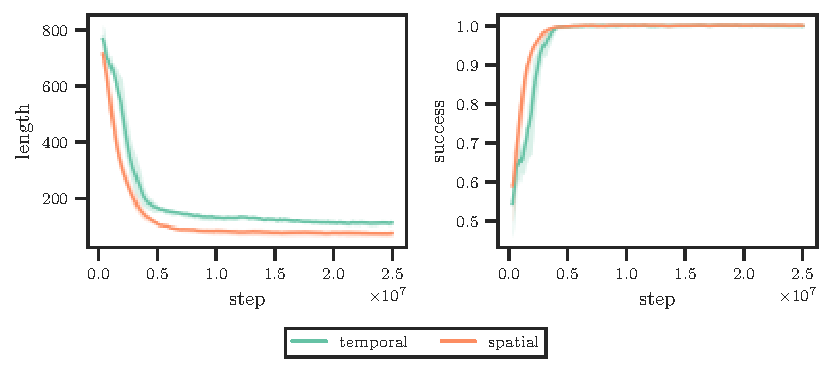
\includegraphics[scale=0.8]{figures/shape-10.pdf}
    \end{figure}
\end{frame}

\begin{frame}
    \begin{figure}
        \centering
        \(15 \times 15\)
        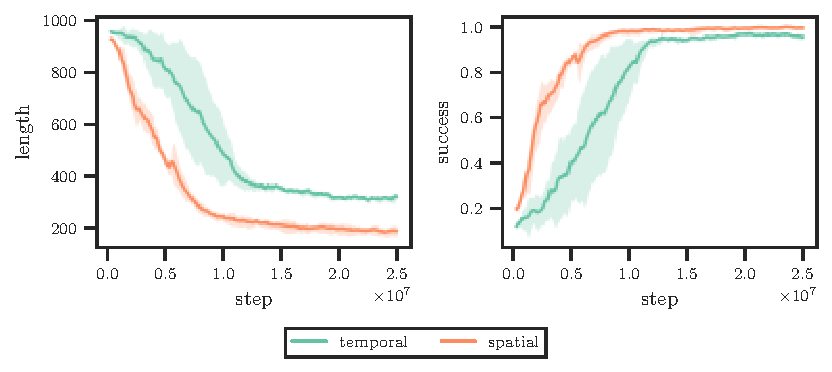
\includegraphics[scale=0.8]{figures/shape-15.pdf}
    \end{figure}
\end{frame}

\begin{frame}
    \begin{figure}
        \centering
        \(20 \times 20\)
        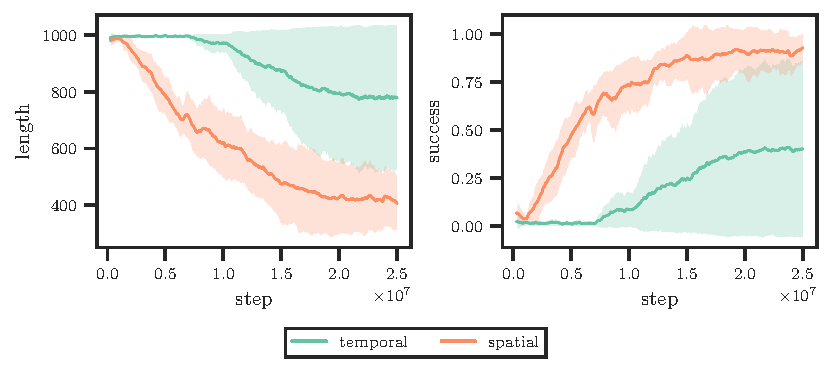
\includegraphics[scale=0.8]{figures/shape-20.pdf}
    \end{figure}
\end{frame}

\subsection{Generalization From Limited Samples}

\begin{frame}
    \frametitle{Experiment III: Generalization From Limited Samples}

    \begin{itemize}
        \item Real-world tasks usually have limited training samples.
        \item Train on 500, 1 000, 5 000 and 10 000 samples of terrain environment.
        \item Test on held out samples from full distribution.
        % high appearance variance and somewhat realistic.
        %Fix seed pool used to generate scenes seen during training.
    \end{itemize}
\end{frame}

\begin{frame}
    \begin{figure}
        \centering
        10000 samples
        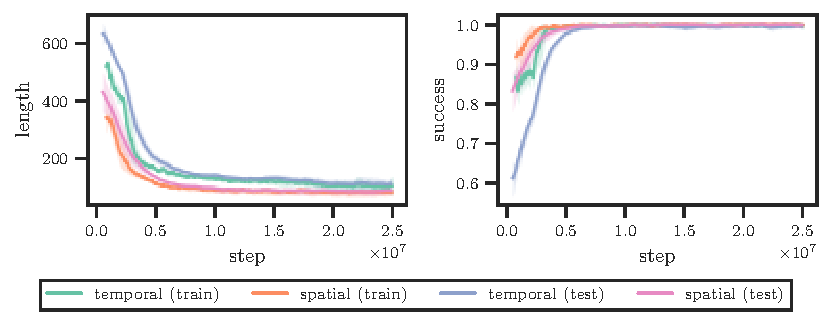
\includegraphics[scale=0.8]{figures/sample-10000.pdf}
    \end{figure}
    % close to full distribution - equal training and test performance for both agents. seemingly no overfitting and good generalization.
\end{frame}

\begin{frame}
    \begin{figure}
        \centering
        5000 samples
        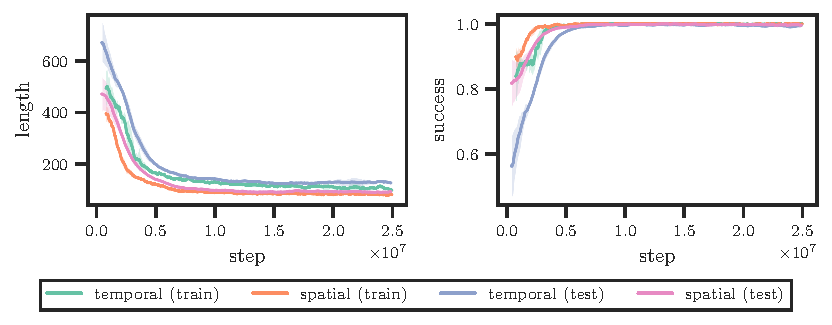
\includegraphics[scale=0.8]{figures/sample-5000.pdf}
    \end{figure}
\end{frame}

\begin{frame}
    \begin{figure}
        \centering
        1000 samples
        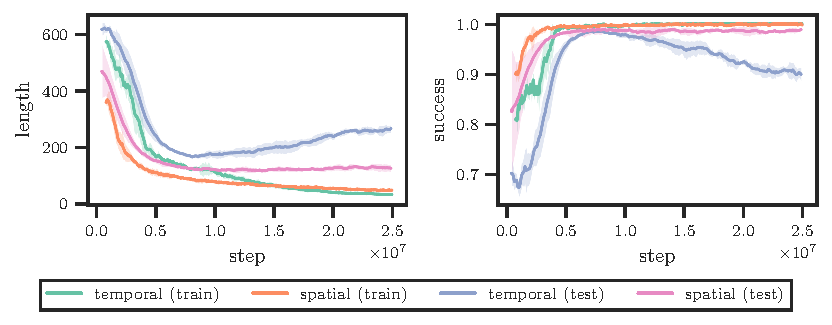
\includegraphics[scale=0.8]{figures/sample-1000.pdf}
    \end{figure}
\end{frame}

\begin{frame}
    \begin{figure}
        \centering
        500 samples
        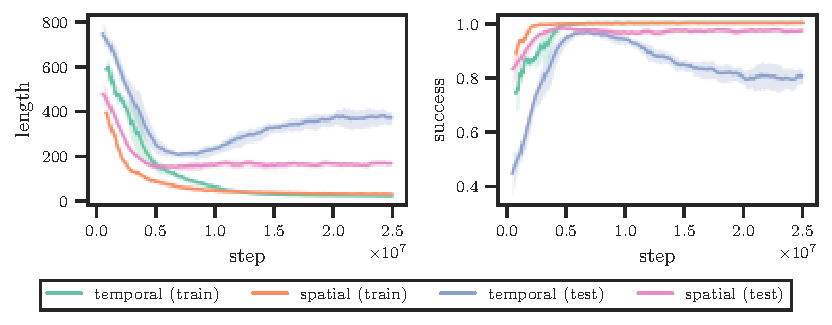
\includegraphics[scale=0.8]{figures/sample-500.pdf}
    \end{figure}
\end{frame}